\documentclass[10pt,a4paper]{standalone}
\usepackage[utf8]{inputenc}
\usepackage{standalone}
\usepackage[T1]{fontenc}
\usepackage[ngerman]{babel}
\usepackage{libertine}
\usepackage{tikz}
\begin{document}
\begin{tikzpicture}[scale=10,font=\small]
\node[anchor=south west,inner sep=0] (image) at (0,0) {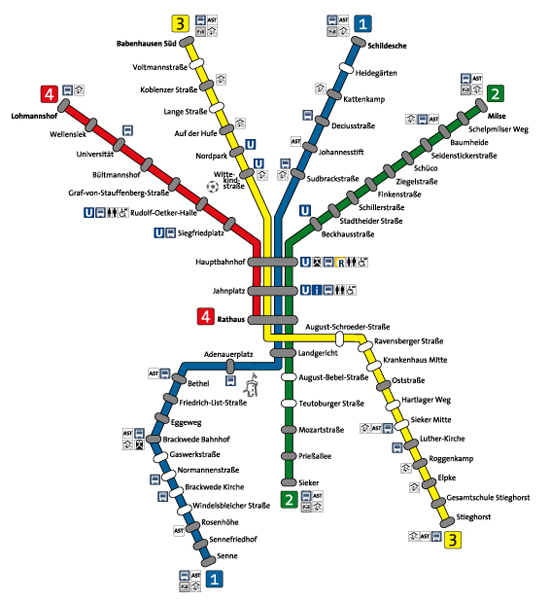
\includegraphics[width=0.9\textwidth]{netzschema.jpg}};
\begin{scope}[x={(image.south east)},y={(image.north west)}]
\draw[help lines,xstep=.01,ystep=.01,gray,very thin] (0,0) grid (1,1);
\foreach \x in {0,1,...,9} { \node [anchor=north] at (\x/10,0) {0.\x}; }
\foreach \y in {0,1,...,9} { \node [anchor=east] at (0,\y/10) {0.\y}; }


%\draw[help lines,xstep=.1,ystep=.1,thick,black] (0,0) grid (1,1);
%\foreach \x in {0,1,...,9} { \node [anchor=north] at (\x/10,0) {0.\x}; }
%\foreach \y in {0,1,...,9} { \node [anchor=east] at (0,\y/10) {0.\y}; }

\tikzstyle{station} = [draw,black,circle,fill=white, inner sep=2pt]
\tikzstyle{outline} = [draw,thick,black,double distance=1.4pt,rounded corners=5pt]
\tikzstyle{inner} = [draw,semithick, #1,line width=1.6pt,rounded corners=5pt]


%Linie 4
\node at (0.116,0.825) (Lohmannshof) {};
\node at (0.1661,0.792) (Wellensiek) {};
\node at (0.2165,0.759) (Uni) {};
\node at (0.267,0.726) (Bültmannshof) {};
\node at (0.317,0.694) (GVS){};
\node at (0.367,0.661) (ROH){};
\node at (0.417,0.628) (Siggi){};
\node at (0.4668,0.595) (HBF4h){};
\node at (0.4668,0.565) (HBF4){};
\node at (0.4668,0.517) (Jahnplatz4){};
\node at (0.4668,0.4685) (Rathaus4){};

\draw[outline] (Lohmannshof.center) -- (Siggi.center) .. controls (HBF4h) .. (HBF4.center) -- (Rathaus4.center);
\draw[inner=red] (Lohmannshof.center) -- (Siggi.center) .. controls (HBF4h) .. (HBF4.center) -- (Rathaus4.center);

\node[station,label=above:Lohmannshof] at (0.116,0.825) (Lohmannshof) {};
\node[station,label=left:Rathaus] at (0.4668,0.4685) (Rathaus4){};

%Line 3
\node at (0.34,0.93) (BHS){};
\node at (0.43,0.749) (Nordpark){};
\node at (0.449,0.712) (WKS){};
\node at (0.486,0.64) (HBF3h){};
\node at (0.486,0.565) (HBF3){};
\node at (0.486,0.517) (Jahnplatz3){};
\node at (0.486,0.4685) (Rathaus3){};
\node at (0.617, 0.438) (ASS){}; 
\node at (0.658, 0.438) (Ravensbergerh){};
\node at (0.67, 0.42) (Ravensberger){};
\node at (0.681, 0.392) (KKHM) {};
\node at (0.813,0.133)(Stieghorst){};


\draw[outline] (BHS.center) -- (WKS.center) .. controls (HBF3h.center) .. (HBF3.center) -- (Rathaus3.center) |- (ASS.east) .. controls (Ravensbergerh) .. (KKHM.center) -- (Stieghorst.center);

\draw[inner=yellow] (BHS.center) -- (WKS.center) .. controls (HBF3h.center) .. (HBF3.center) -- (Rathaus3.center) |- (ASS.east) .. controls (Ravensbergerh) .. (KKHM.center) -- (Stieghorst.center);

\node[station,label=above:Babenhausen Süd] at (0.34,0.93) (BHS){};
\node[station,label=below:Stieghorst]at (0.813,0.133)(Stieghorst){};

%linie 2
%\node[station]

\node at (0.875,0.825)(Milse){};
\node at (0.573,0.626)(Beckhausstrasse){};

\node at (0.526,0.61) (HBF2h){};
\node at (0.526,0.565) (HBF2){};
\node at (0.526,0.517) (Jahnplatz2){};
\node at (0.526,0.4685) (Rathaus2){};

\node at (0.525,0.2) (Sieker) {};

\draw[outline] (Milse.center) .. controls (Beckhausstrasse.center) and (HBF2h).. (HBF2.center) -- (Sieker.center);
\draw[inner=green] (Milse.center) .. controls (Beckhausstrasse.center) and (HBF2h).. (HBF2.center) -- (Sieker.center);

\node[station,label=above:Milse] at (0.875,0.825)(Milse){};
\node[station,label=below:Sieker] at (0.525,0.2) (Sieker) {};

%linie1
\node[station] at (0.652,0.93) (Schildesche){};
\node at (0.541,0.71) (SBS){};


\node at (0.505,0.64) (HBF1h){};
\node at (0.505,0.565) (HBF1){};
\node at (0.505,0.517) (Jahnplatz1){};
\node at (0.505,0.4685) (Rathaus1){};

\node at (0.418,0.392)(Adenauerplatz){};

\node at (0.325,0.371)(Bethel){};
\node at (0.333,0.392)(Bethelh){};
\node at (0.28,0.271) (BWBH){};

\node at (0.38,0.068) (Senne){};

\draw[outline] (Schildesche.center) -- (SBS.center) .. controls (HBF1h) .. (Jahnplatz1.center) |- (Adenauerplatz.center) -- (Bethelh.center) -- (BWBH.center) -- (Senne.center);

\draw[inner=blue] (Schildesche.center) -- (SBS.center) .. controls (HBF1h) .. (Jahnplatz1.center) |- (Adenauerplatz.center) -- (Bethelh.center) -- (BWBH.center) -- (Senne.center);

\node[station,label=above:Schildesche] at (0.652,0.93) (Schildesche){};
\node[station,label=below:Senne] at (0.38,0.068) (Senne){};

\end{scope}
\end{tikzpicture}
\end{document}